{\usebackgroundtemplate{
  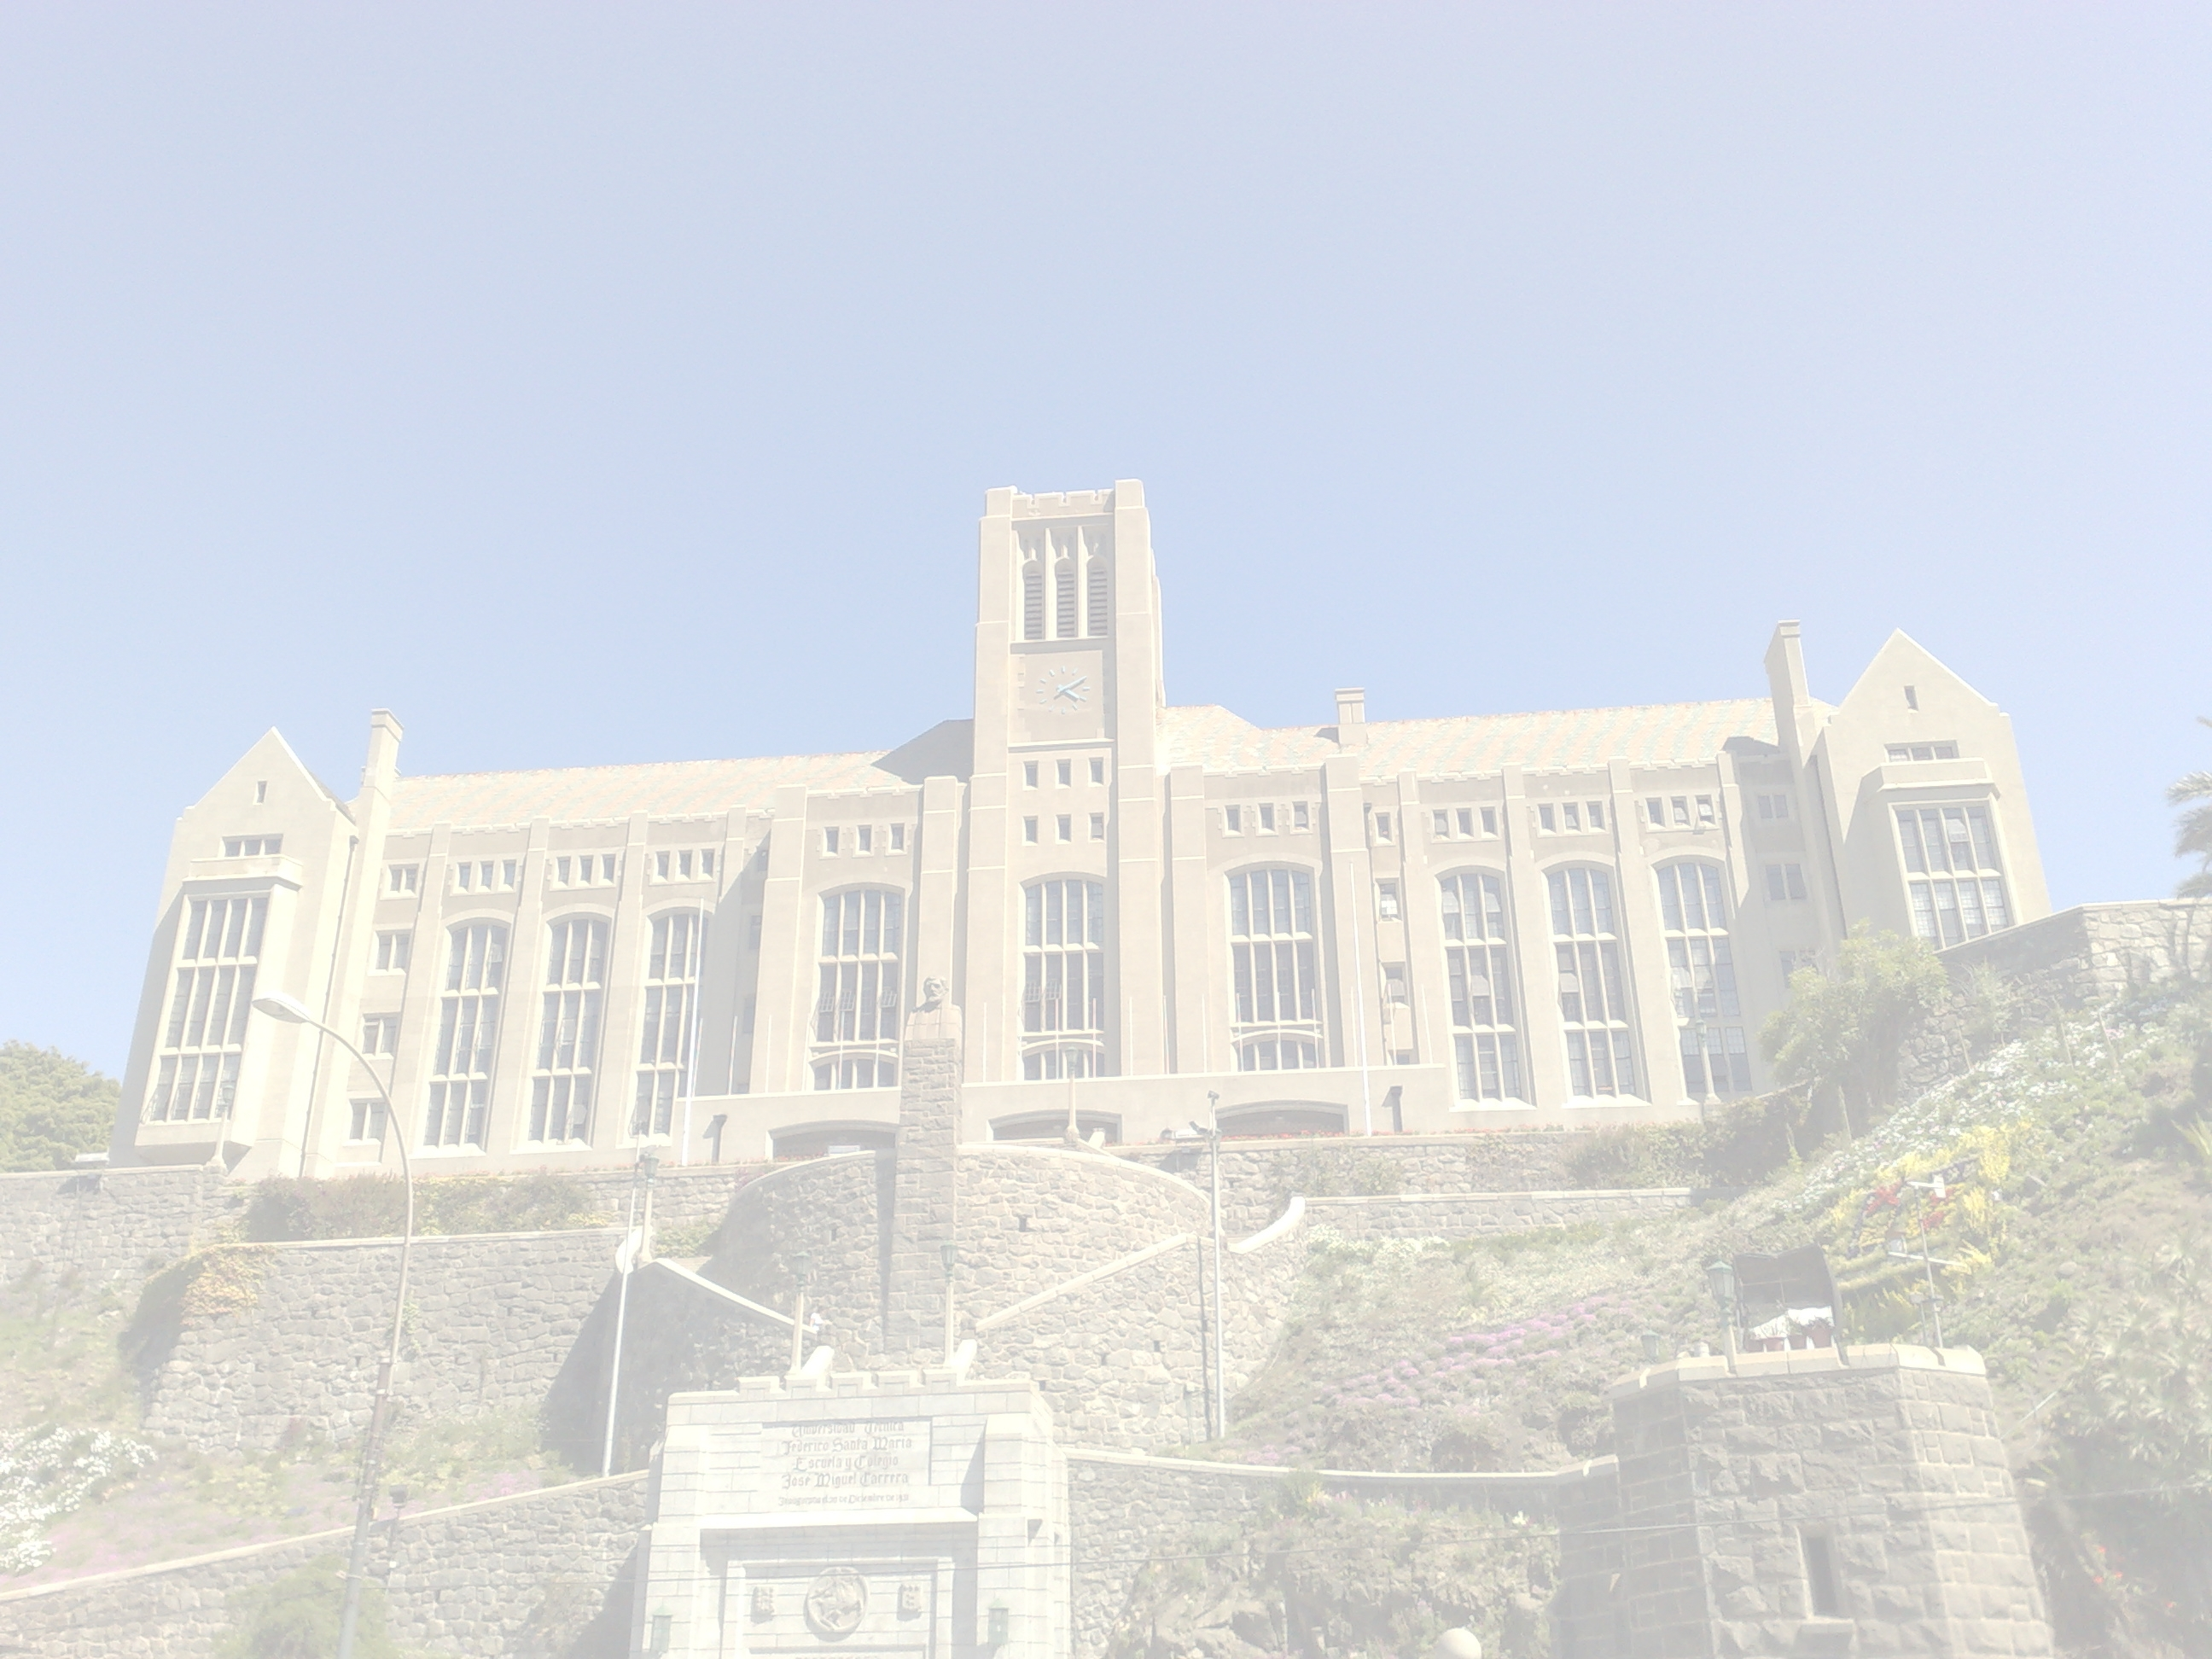
\includegraphics[width=\paperwidth,
    height=\paperheight]{Pict/UTFSM-30.jpg}
}
  \begin{frame}
    \titlepage
  \end{frame}
}


\begin{frame}
  \frametitle{More about the metric}
  \begin{columns}[t]
    \column{.45\textwidth}
    The metric
    \begin{itemize}
    \item  is defined to be a symmetric $\binom{0}{2}$-tensor
    \item relate the vectors and covectors.
    \item define distance.
    \item with upper indices denotes the inverse of the metric.
    \item with mixed indices is \alert{always} a Kr\"onecker delta.
    \end{itemize}
    \column{.45\textwidth}
    \begin{block}{Metric and vector basis}
      Given a set of vector basis, $\{\vb{i}\}$, the metric can be obtain though the relation,
      \begin{align*}
        g_{i j} = \vb{i}\cdot \vb{j}
      \end{align*}
    \end{block}
  \end{columns}
\end{frame}




{\usebackgroundtemplate{
    
\includegraphics[width=\paperwidth,
      height=\paperheight]{Pict/Q2.pdf}
  }
\begin{frame}
  \frametitle{\alert{WORKED EXAMPLES}}
  A metric can be viewed as a linear map between the tangent and cotangent space,
  \begin{align*}
    g:TM\to T^*M.
  \end{align*}
  \begin{itemize}[<+-|alert@+>]
  \item Given a vector $V^i=\(V^x,V^y,V^z\)$ in a space with Euclidean metric. Find the associated covector.
  \item Given a vector $V^i=\(V^r,V^\theta,V^\varphi\)$ in a space with polar metric. Find the associated covector.
  \end{itemize}
\end{frame}
}

\begin{frame}
  \frametitle{Lorentzian Metrics}
  \begin{columns}[t]
    \column{.45\textwidth}
    \begin{itemize}
    \item If one of the signs defining the line element of the metric is not positive, the metric is said to be \alert{Lorentzian}
    \item The spacetime admits a Lorentzian metric.
    
    \end{itemize}
    \column{.45\textwidth}
    \begin{itemize}
    \item  The \alert{Minkowskian} metric is the equivalent to Euclidean, but for Lorentzian spaces.
    \end{itemize}
    \begin{align*}
      ds^2(\eta) = -dt^2+dx^2+dy^2+dz^2
    \end{align*}
  \end{columns}

  \begin{alertblock}{Lack of positivity}
    Vectors in Lorentzian spaces, do not have positive norm. However, there exist three type of vectors, accordingly to their norm: space-like ($|{\vec{V}}|>0$), time-like ($|{\vec{V}}|<0$) and null-like ($|{\vec{V}}|=0$)
  \end{alertblock}
\end{frame}

\begin{frame}
  \frametitle{Levi-Civita Epsilon}
  \begin{columns}[t]
  \column{.4\textwidth}
  \begin{itemize}
  \item Its rank is equal to the dimension of the space
  \item Totally antisymmetric
  \item It has a single independent component
  \end{itemize}
  \column{.6\textwidth}
  \begin{definition}{Levi-Civita epsilon}
    \begin{align*}
      \epsilon_{a_1 \cdots a_n} =
      \begin{cases}
        1 & 
        {\tiny \begin{pmatrix}
          1&\cdots&n\\
          a_1& \cdots& a_n
        \end{pmatrix}}
        \text{ is even}\\
        -1 & 
        {\tiny \begin{pmatrix}
          1&\cdots&n\\
          a_1& \cdots& a_n
        \end{pmatrix}}\
        text{ is odd}\\
        0 & \text{otherwise}
      \end{cases}
    \end{align*}
  \end{definition}
  \end{columns}
  \begin{alertblock}{IMPORTANT NOTE}
    In Minkowskian spaces, $$\epsilon^{a_1 \cdots a_n}=-\epsilon_{a_1 \cdots a_n},$$due to the different sign of the ``time''-like dimension.
  \end{alertblock}
\end{frame}


{\usebackgroundtemplate{
    
\includegraphics[width=\paperwidth,
      height=\paperheight]{Pict/Q2.pdf}
  }
\begin{frame}
  \frametitle{\alert{WORKED EXAMPLES}}
  \begin{itemize}[<+-|alert@+>]
  \item Vector product of vectors (defined only on $\R^3$)
  \item Let $M$ be a 3 by 3 matrix. Show that $\epsilon^{abc} M_{1a}M_{2b}M_{3c}$ is the determinant of $M$.
  \end{itemize}
\end{frame}
}

\begin{frame}
  \frametitle{Useful Identity (super saiyajin)}
  \begin{columns}
    \column{.75\textwidth}
    \begin{alertblock}{Epsilon ``Product''}
      \begin{align*}
        \epsilon^{a_1 \cdots a_n}\epsilon_{b_1 \cdots b_n}=
        \begin{vmatrix}
          \delta^{a_1}_{b_1} &\cdots&\delta^{a_1}_{b_n}\\
          \vdots & & \vdots \\
          \delta^{a_n}_{b_1}& \cdots & \delta^{a_n}_{b_n}
        \end{vmatrix}
      \end{align*}
    \end{alertblock}

    \begin{block}{Corollary}
      \begin{align*}
        \epsilon^{a_1 \cdots a_p c_{p+1}\cdots c_n}\epsilon_{b_1 \cdots b_p c_{p+1}\cdots c_n}= (n-p)!
        \begin{vmatrix}
          \delta^{a_1}_{b_1} &\cdots&\delta^{a_1}_{b_p}\\
          \vdots & & \vdots \\
          \delta^{a_p}_{b_1}& \cdots & \delta^{a_p}_{b_p}
        \end{vmatrix}
      \end{align*}
    \end{block}

    \column{.25\textwidth}
    \begin{center}
      
\includegraphics[scale=.25]{Pict/Goku_super_saiyajin_2.png}
    \end{center}
  \end{columns}
\end{frame}

\begin{frame}
  \frametitle{$\epsilon $ is not a tensor!}
  \begin{columns}
    \column{.55\textwidth}
    Let $M$ be a matrix, then 
    \begin{align*}
      \epsilon_{a_1\cdots a_n} \det(M) = \epsilon_{b_1\cdots b_n} M_{a_1}^{b_1}\cdots M_{a_n}^{b_n}.
    \end{align*}
    
    Therefore,  $\epsilon$ does not transform with a ``matrix'' for each index, instead includes a factor proportional to the determinant of $M$
    \column{.4\textwidth}   
    \begin{definition}
      A \alert{tensor density} of order $\omega$, transform as a tensor, but includes a factor of $\abs{\det{M}}^\omega$.
    \end{definition}
  \end{columns}

  \begin{alertblock}{Formally...}
    The Levi-Civita epsilon is a tensor density of rank $n$ and order one.
  \end{alertblock}
\end{frame}

\begin{frame}
  \frametitle{Fundamental Problem}
  \begin{description}
  \item[Question] How is it possible to compare vectors that do not lie on the the same point in space?
  \item [\alert{Answer}] It is not possible! Unless a way to transport the vector to the same point is defined.

    This objects are known as \alert{connections}.
  \end{description}
\end{frame}

\begin{frame}
  \frametitle{Connection and Covariant derivative}

  \begin{columns}
    \column{.45\textwidth}
    Consider a vector $\vec{V}=V^a\vb{a}$. 

    Then its derivative is,
    \begin{align*}
      \partial_b\vec{V} &= (\partial_bV^a)\vb{a} + V^a (\partial_b\vb{a})\\
      &= (\partial_bV^a)\vb{a} + V^a \Gamma_{ba}^c \vb{c}\\
      &= (\partial_bV^c)\vb{c} + V^a \Gamma_{ba}^c \vb{c}\\
      &= \(\partial_bV^c + V^a \Gamma_{ba}^c\) \vb{c}\\
      &= \(\covd_b V\)^c\vb{c}
    \end{align*}
    \column{.45\textwidth}
    \onslide<2>{
      \begin{itemize}
      \item $\Gamma$ is known as the connection, in this case defined through
        \begin{align*}
          \Gamma_{ba}^c \vb{c}= \partial_b \vb{a}.
        \end{align*}
      \item $\covd_b$ is the covariant derivative.
      \end{itemize}
    }
  \end{columns}
\end{frame}

\begin{frame}
  \frametitle{Levi-Civita Connection}
 
  The Levi-Civita connection is symmetric in the lower indices.

  A covariant derivative is defined with this connection, s.t.
  \begin{align*}
    \covd:C^\infty(\otimes^p TM\otimes^q T^*M) \to C^\infty(\otimes^p TM\otimes^{q+1} T^*M)
  \end{align*}

  \begin{alertblock}{WARNING!!!}
    Physicists and Mathematicians do not use the same language, in general!
  \end{alertblock}
\end{frame}

{\usebackgroundtemplate{
    
\includegraphics[width=\paperwidth,
      height=\paperheight]{Pict/Q2.pdf}
  }
\begin{frame}
  \frametitle{\alert{WORKED EXAMPLES}}
  \begin{itemize}%[<+-|alert@+>]
  \item How do the connection transform?
    \onslide<2>{
      \begin{alertblock}{Not a tensor!!!}
        The transformation rule of the connection is not the one for a rank 3 tensor. Moreover, a geometrical object which transform this way, is said to be a connection!!!
      \end{alertblock}
    }
  \item Use the Leibniz rule to show how the covariant derivative act on 
    \begin{itemize}
    \item scalars
    \item covectors
    \item tensor of rank 2 (like the metric)
    \end{itemize}
  \end{itemize}
\end{frame}
}

\begin{frame}
  \frametitle{Compatibility with the metric}
  \begin{columns}
    \column{.45\textwidth}
    \uline{Condition:}
    \begin{align*}
      \covd_a g_{bc} =0
    \end{align*}
    \uline{Consequence:}
    \begin{itemize}
    \item Commutation of contraction and derivation.
    \end{itemize}
    \column{.45\textwidth}
    \begin{alertblock}{WORKED EXAMPLE}
      Assuming the metric compatibility and symmetry on the lower indices of the connection. Find the definition of  $\Gamma$ as a function of the metric.
    \end{alertblock}
  \end{columns}
\end{frame}
